\documentclass[aspectratio=169]{beamer}

% ============================================================
%  Dynamic Louvain on GPUs with CUDA  --  B.Tech Project
%  Raadhes Chandaluru  |  under Prof. Rupesh Nasre  |  IIT Madras
% ============================================================

% - THEME (matches the UGRC deck) -
\usetheme{Madrid}
\usecolortheme{beaver}
\setbeamertemplate{navigation symbols}{}
\setbeamertemplate{caption}{\raggedright\insertcaption\par}

% - PACKAGES -
\usepackage[T1]{fontenc}
\usepackage{lmodern}
\usepackage{tikz}
\usetikzlibrary{shapes, arrows.meta, positioning, fit, backgrounds, calc, shadows}
\usepackage{pgfplots}
\pgfplotsset{compat=1.18}
\usepgfplotslibrary{groupplots}
\usepackage{booktabs}
\usepackage{amsmath}

% - community colours (match the report) -
\definecolor{cBlue}{RGB}{197,217,241}
\definecolor{cOrange}{RGB}{252,224,196}
\definecolor{cGreen}{RGB}{205,232,205}

% short helper for "win" / "loss" cells
\newcommand{\win}[1]{\textcolor{green!50!black}{\textbf{#1}}}
\newcommand{\loss}[1]{\textcolor{red!70!black}{#1}}

% - METADATA -
\title[Dynamic Louvain on GPUs]{Dynamic Louvain on GPUs with CUDA}
\subtitle{B.Tech Project - Final Presentation}
\author[Raadhes Ch.]{Raadhes Chandaluru \\ \small Under Prof.\ Rupesh Nasre}
\institute[IIT Madras]{Department of Computer Science and Engineering \\ Indian Institute of Technology Madras}
\date{June 2026}

% - section divider: a "you are here" outline at the start of each section -
\AtBeginSection[]{%
  \begin{frame}{Overview}
    \tableofcontents[currentsection]
  \end{frame}
}

\begin{document}

% ============================================================
% TITLE + OUTLINE
% ============================================================
\begin{frame}
    \titlepage
\end{frame}

\begin{frame}{Overview}
    \tableofcontents
\end{frame}

% ============================================================
\section{Introduction}
% ============================================================

\begin{frame}{Graphs are Everywhere}
    \centering
    Almost every modern system is a \textbf{network} of \textbf{vertices} and \textbf{edges}:
    \vspace{0.3em}

    \begin{columns}[T]
        \column{0.32\textwidth}\centering
        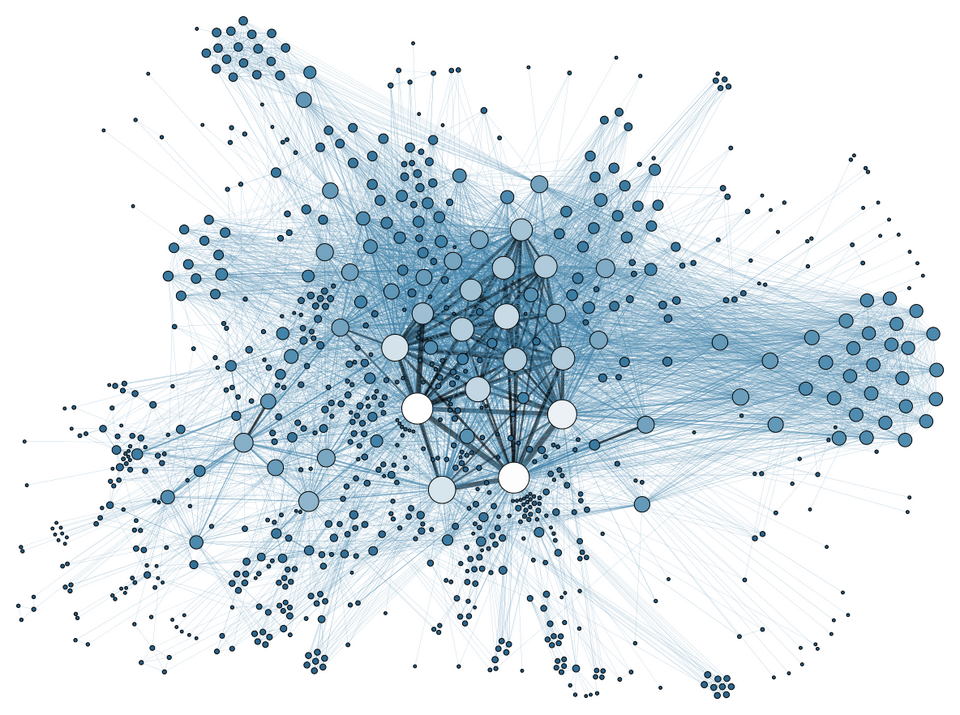
\includegraphics[height=2.4cm,keepaspectratio]{images/net_social.png}\\[0.2em]{\scriptsize Social networks}
        \column{0.32\textwidth}\centering
        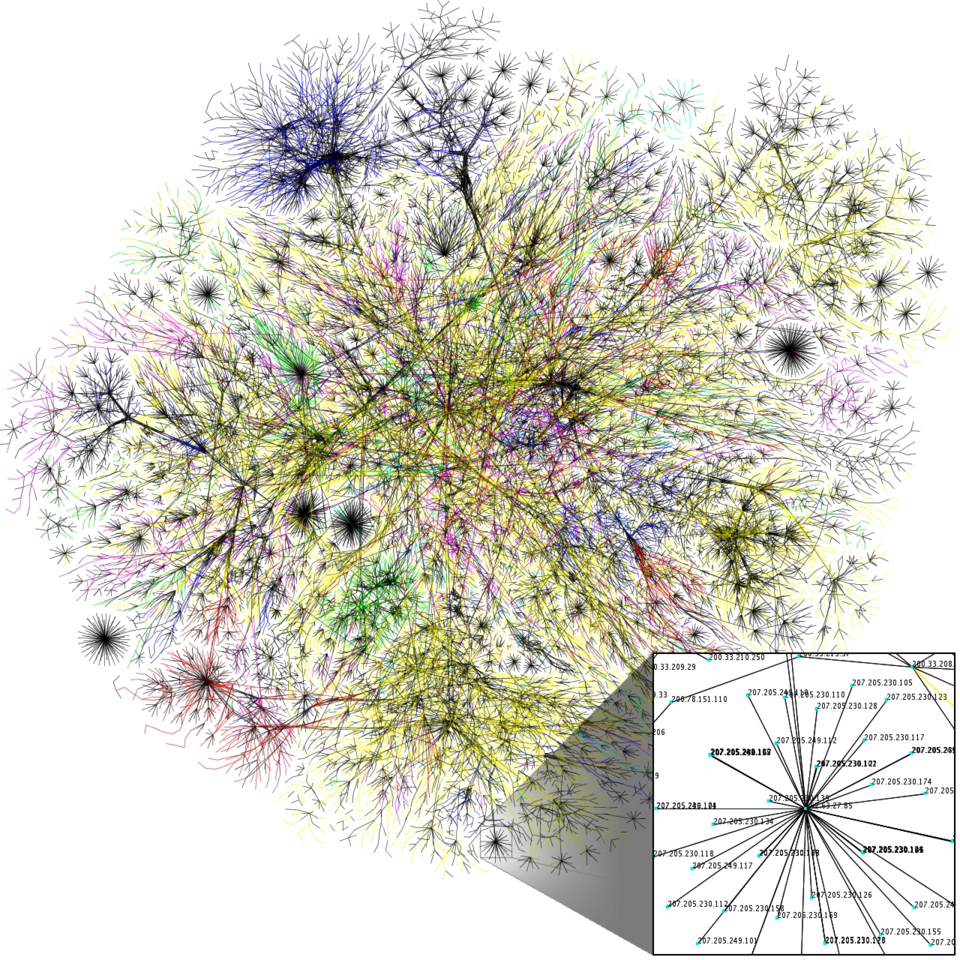
\includegraphics[height=2.4cm,keepaspectratio]{images/net_web.png}\\[0.2em]{\scriptsize The web / internet}
        \column{0.32\textwidth}\centering
        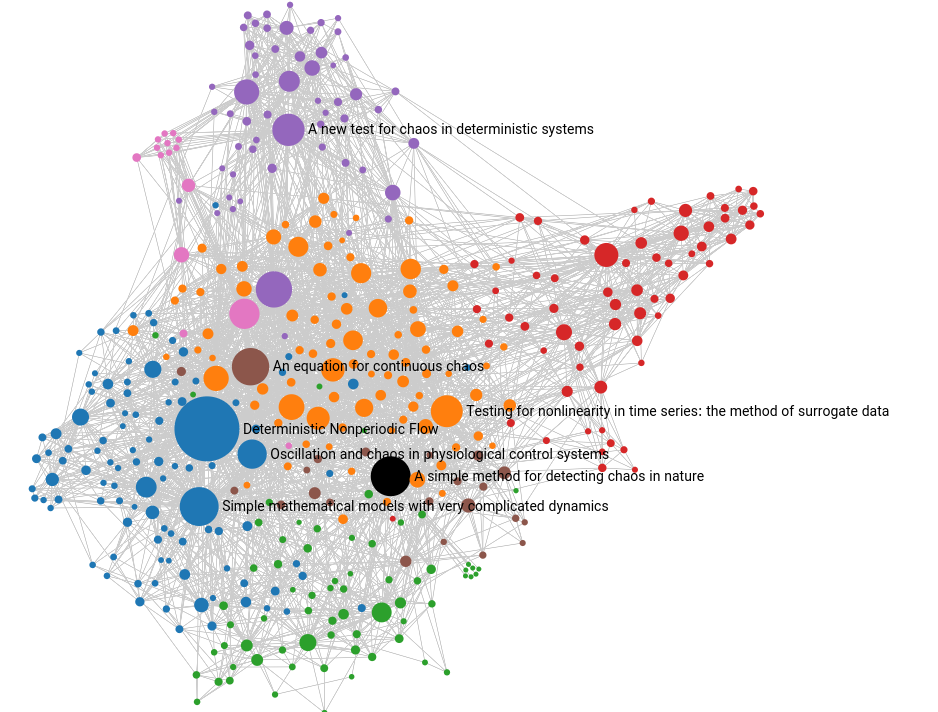
\includegraphics[height=2.4cm,keepaspectratio]{images/net_citations.png}\\[0.2em]{\scriptsize Citation networks}
    \end{columns}
    \vspace{0.5em}

    \begin{columns}[T]
        \column{0.32\textwidth}\centering
        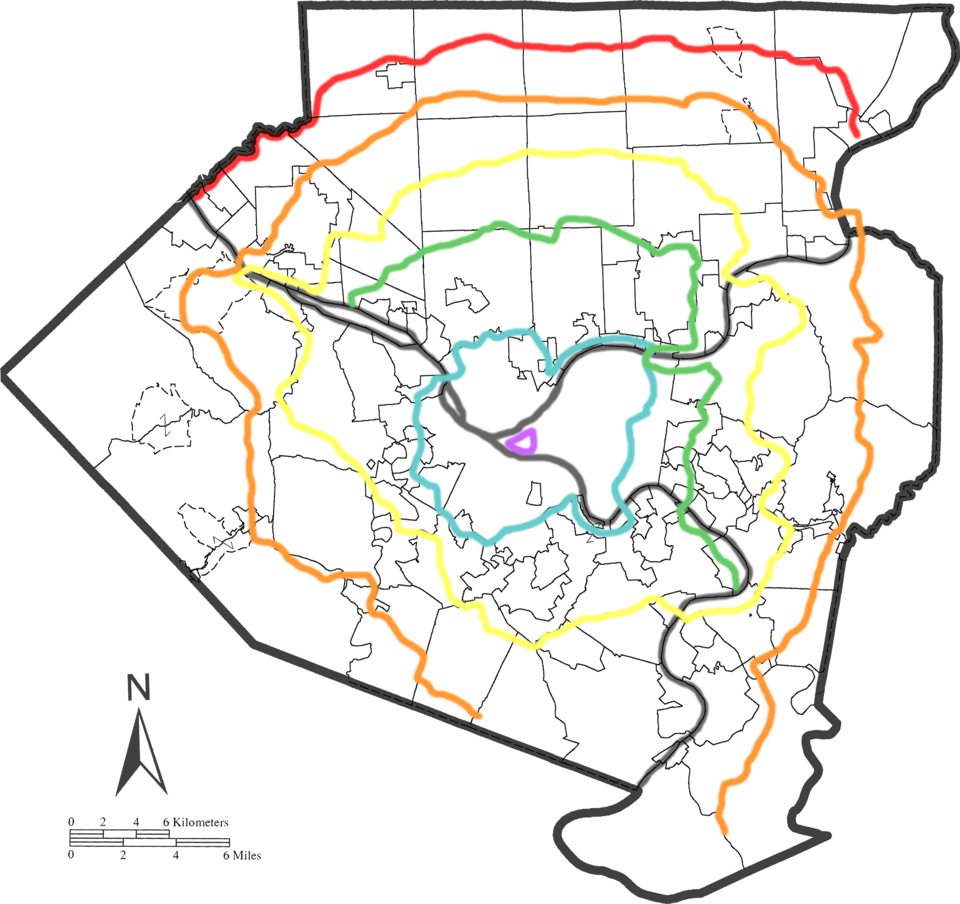
\includegraphics[height=2.4cm,keepaspectratio]{images/net_roads.png}\\[0.2em]{\scriptsize Road networks}
        \column{0.32\textwidth}\centering
        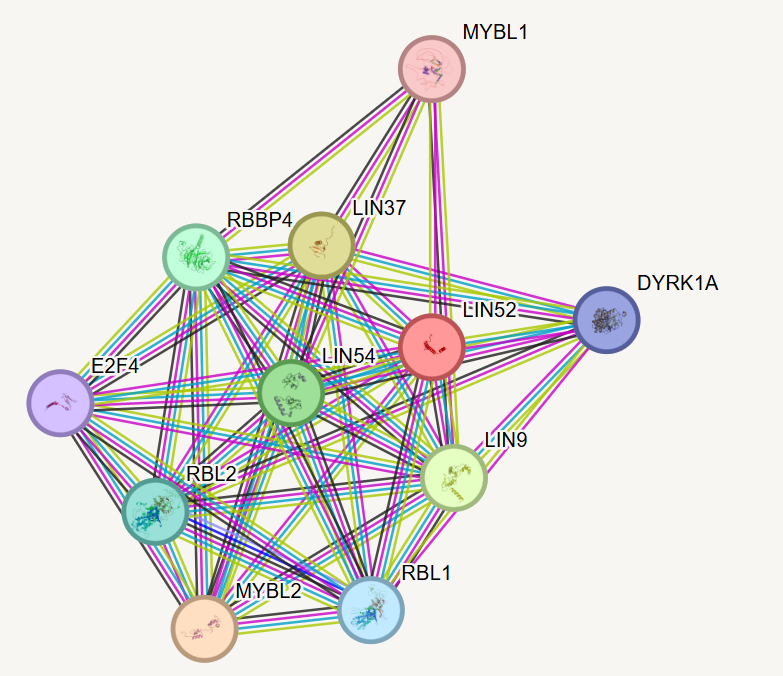
\includegraphics[height=2.4cm,keepaspectratio]{images/net_biology.png}\\[0.2em]{\scriptsize Protein interactions}
        \column{0.32\textwidth}\centering
        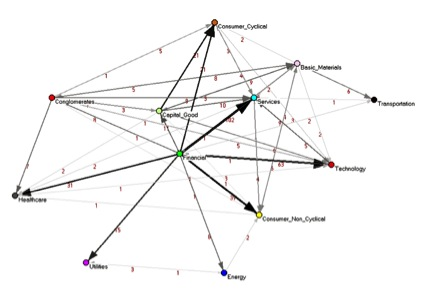
\includegraphics[height=2.4cm,keepaspectratio]{images/net_finance.jpg}\\[0.2em]{\scriptsize Financial networks}
    \end{columns}
    \vfill
    {\tiny Images: Wikimedia Commons (CC).}
\end{frame}

\begin{frame}{Community Detection}
    \begin{columns}
        \column{0.56\textwidth}
        \begin{itemize}
            \item \textbf{Community detection} partitions the vertices into groups that are
            \textbf{densely connected inside} and \textbf{sparsely connected outside}.
            \item These groups carry meaning - friend circles, topical web pages, functional
            protein modules.
            \item Powers \textbf{influence maximisation}, \textbf{fraud detection},
            \textbf{recommendation}, and \textbf{protein-function prediction}.
        \end{itemize}
        \column{0.44\textwidth}
        \centering
        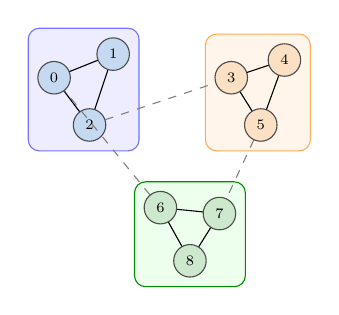
\begin{tikzpicture}[scale=0.75, transform shape,
            v/.style={circle, draw=black!70, minimum size=5.5mm, inner sep=0pt, font=\scriptsize}]
            \node[v, fill=cBlue]   (0) at (0,2)    {0};
            \node[v, fill=cBlue]   (1) at (1,2.4)  {1};
            \node[v, fill=cBlue]   (2) at (0.6,1.2){2};
            \node[v, fill=cOrange] (3) at (3,2)    {3};
            \node[v, fill=cOrange] (4) at (3.9,2.3){4};
            \node[v, fill=cOrange] (5) at (3.5,1.2){5};
            \node[v, fill=cGreen]  (6) at (1.8,-0.2){6};
            \node[v, fill=cGreen]  (7) at (2.8,-0.3){7};
            \node[v, fill=cGreen]  (8) at (2.3,-1.1){8};
            \draw (0)--(1) (1)--(2) (2)--(0);
            \draw (3)--(4) (4)--(5) (5)--(3);
            \draw (6)--(7) (7)--(8) (8)--(6);
            \draw[gray, dashed] (2)--(3) (5)--(7) (6)--(0);
            \begin{scope}[on background layer]
              \node[draw=blue!55, fill=blue!7, rounded corners, fit=(0)(1)(2)] {};
              \node[draw=orange!65, fill=orange!8, rounded corners, fit=(3)(4)(5)] {};
              \node[draw=green!55!black, fill=green!7, rounded corners, fit=(6)(7)(8)] {};
            \end{scope}
        \end{tikzpicture}
        \\[0.3em]
        {\scriptsize Dense inside, sparse between.}
    \end{columns}
\end{frame}

% ============================================================
\section{The Louvain Algorithm}
% ============================================================

\begin{frame}{Modularity - the Objective}
    \textbf{Modularity $Q$} scores a partition: observed intra-community edge fraction
    \emph{minus} what we'd expect at random.
    \[
        Q = \frac{1}{2m}\sum_{i,j}\left[A_{ij} - \frac{k_i k_j}{2m}\right]\delta(c_i,c_j)
        \qquad\in[-0.5,\,1],\ \text{higher is better}
    \]
    Equivalently, as a sum of \textbf{per-community} contributions:
    \[
        Q = \sum_c Q_c, \qquad
        Q_c = \frac{\Sigma_{in}(c)}{2m} - \left(\frac{\Sigma_{deg}(c)}{2m}\right)^{2}
    \]
    \begin{itemize}\small
        \item $m$: total edge weight \quad $A_{ij}$: edge weight \quad $k_i$: weighted degree
        \item $\Sigma_{in}(c)$: edges inside $c$ \quad $\Sigma_{deg}(c)$: total degree of $c$
        \item $\delta(c_i,c_j)=1$ iff $i,j$ in the same community.
    \end{itemize}
\end{frame}

\begin{frame}{The Louvain Method - Two Repeating Phases}
    \centering
    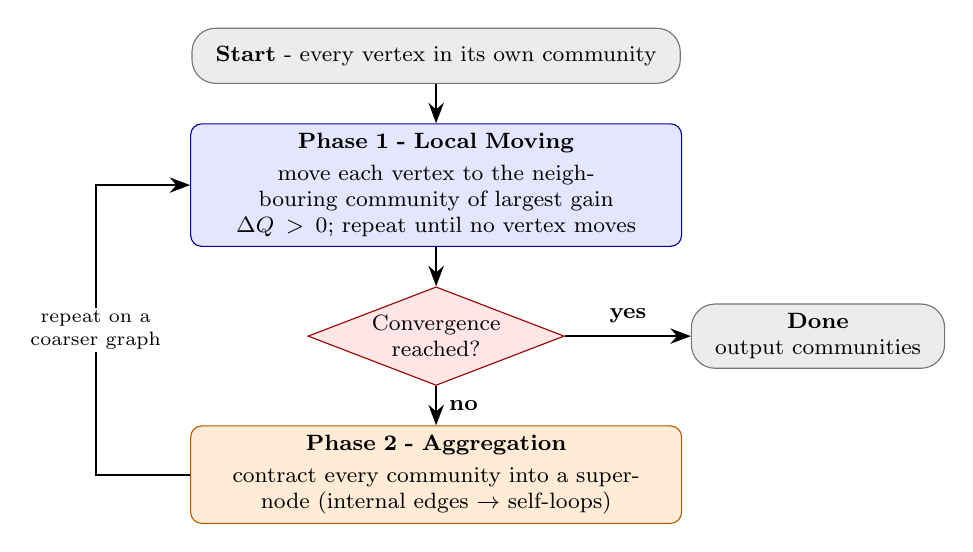
\begin{tikzpicture}[
        font=\footnotesize,
        node distance=5mm and 16mm,
        term/.style={rectangle, rounded corners=3mm, draw=black!55, fill=gray!15,
                     align=center, minimum height=7mm, inner xsep=3mm},
        proc/.style={rectangle, rounded corners, draw=blue!55!black, fill=blue!10,
                     align=center, text width=6.0cm, minimum height=10mm},
        agg/.style={rectangle, rounded corners, draw=orange!70!black, fill=orange!16,
                    align=center, text width=6.0cm, minimum height=10mm},
        dec/.style={diamond, draw=red!60!black, fill=red!10, aspect=2.6,
                    align=center, inner sep=1pt},
        flow/.style={-{Stealth[length=2.6mm]}, thick},
    ]
        \node[term] (start) {\textbf{Start} - every vertex in its own community};
        \node[proc, below=of start] (p1)
            {\textbf{Phase 1 - Local Moving}\\[2pt]
             move each vertex to the neighbouring community of largest gain
             $\Delta Q>0$; repeat until no vertex moves};
        \node[dec, below=of p1] (dec) {Convergence\\reached?};
        \node[agg, below=of dec] (p2)
            {\textbf{Phase 2 - Aggregation}\\[2pt]
             contract every community into a super-node
             (internal edges $\to$ self-loops)};
        \node[term, right=16mm of dec] (stop)
            {\textbf{Done}\\ output communities};

        \draw[flow] (start) -- (p1);
        \draw[flow] (p1) -- (dec);
        \draw[flow] (dec) -- node[right=1pt]{\textbf{no}} (p2);
        \draw[flow] (dec) -- node[above=1pt]{\textbf{yes}} (stop);
        \draw[flow] (p2.west) -- ++(-1.2,0) |- (p1.west);
        \node[font=\scriptsize, align=center, fill=white, inner sep=1pt]
            at ($(p1.west)!0.5!(p2.west) + (-1.2,0)$) {repeat on a\\coarser graph};
    \end{tikzpicture}
\end{frame}

\begin{frame}{Modularity Gain $\Delta Q$}
    Moving node $i$ from community $a$ to community $b$:
    \[
        \Delta Q_{i:a\to b} = \frac{1}{m}\left[(k_{i,b}-k_{i,a})
            - \frac{k_i}{2m}\bigl(k_i + \Sigma_b - \Sigma_a\bigr)\right]
    \]
    \begin{itemize}\small
        \item $k_{i,x}$: weight of edges from $i$ into community $x$
        \item $k_i$: weighted degree of $i$ \qquad $\Sigma_x$: total degree of community $x$
    \end{itemize}
    \vspace{0.4em}
    For a node leaving its \textbf{own singleton} ($k_{i,a}=0,\ \Sigma_a=k_i$) this simplifies to
    \[
        \boxed{\ \Delta Q_{i\to b} = \frac{1}{m}\left[k_{i,b}
            - \frac{k_i\,\Sigma_{deg}(b)}{2m}\right]\ }
    \]
    \centering\small Only \textbf{local} quantities - cheap to evaluate per node.
\end{frame}

\begin{frame}{Worked Example (1/6) - Setup ($m=12$)}
    \begin{columns}
        \column{0.5\textwidth}
        Nine nodes: \textbf{three triangles} joined in a ring by three bridge edges.
        Every node starts in its \textbf{own} community.
        \vspace{0.5em}

        Six bridge nodes have degree $3$, three outer nodes degree $2$:
        \begin{align*}
            Q_0 &= -\frac{1}{(2m)^2}\sum_i k_i^2 \\[2pt]
                &= -\frac{6\cdot 3^2 + 3\cdot 2^2}{24^2}
                 = -\frac{66}{576} \approx -0.115 .
        \end{align*}
        \column{0.5\textwidth}
        \centering
        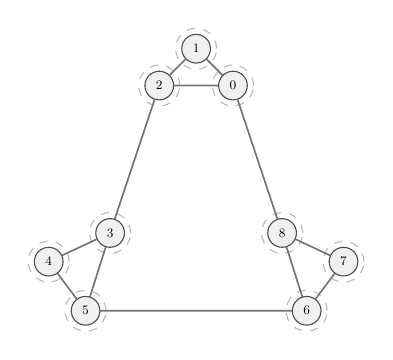
\begin{tikzpicture}[scale=0.52, transform shape,
            vtx/.style={circle, draw=black!70, fill=gray!12, minimum size=7mm, inner sep=0pt, font=\small},
            ed/.style={draw=black!55, semithick},
            sing/.style={draw=gray!55, dashed, circle, minimum size=10mm}]
            \node[vtx] (1) at (0,4)       {1};
            \node[vtx] (2) at (-0.9,3.1)  {2};
            \node[vtx] (0) at (0.9,3.1)   {0};
            \node[vtx] (3) at (-2.1,-0.5) {3};
            \node[vtx] (4) at (-3.6,-1.2) {4};
            \node[vtx] (5) at (-2.7,-2.4) {5};
            \node[vtx] (8) at (2.1,-0.5)  {8};
            \node[vtx] (7) at (3.6,-1.2)  {7};
            \node[vtx] (6) at (2.7,-2.4)  {6};
            \draw[ed] (0)--(1) (1)--(2) (2)--(0);
            \draw[ed] (3)--(4) (4)--(5) (5)--(3);
            \draw[ed] (6)--(7) (7)--(8) (8)--(6);
            \draw[ed] (2)--(3) (5)--(6) (8)--(0);
            \begin{scope}[on background layer]
                \foreach \n in {1,2,0,3,4,5,8,7,6} { \node[sing] at (\n) {}; }
            \end{scope}
        \end{tikzpicture}
    \end{columns}
\end{frame}

\begin{frame}{Worked Example (2/6) - Local Moving: Node 1}
    \begin{columns}
        \column{0.46\textwidth}
        \small
        Every node sits in its \textbf{own community} (dashed circles).
        \textbf{Node 1} ($k_1{=}2$) tests its two neighbours $\{0\}$ and $\{2\}$:
        \begin{align*}
            \Delta Q_{1\to\{0\}} &= \tfrac{1}{12}\!\left[1-\tfrac{2\cdot3}{24}\right]=0.0625\\[1pt]
            \Delta Q_{1\to\{2\}} &= \tfrac{1}{12}\!\left[1-\tfrac{2\cdot3}{24}\right]=0.0625
        \end{align*}
        Both are $>0$ and \emph{equal}; the tie is broken arbitrarily, so node 1 joins $\{0\}$.
        \column{0.54\textwidth}
        \centering
        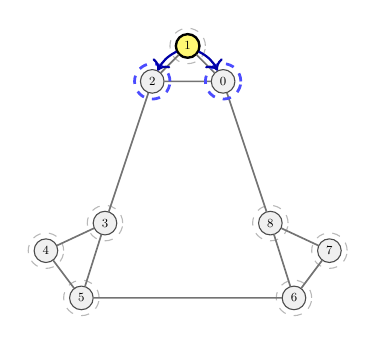
\begin{tikzpicture}[scale=0.5, transform shape,
            vtx/.style={circle, draw=black!70, fill=gray!12, minimum size=6mm, inner sep=0pt, font=\small},
            ed/.style={draw=black!55, semithick},
            sing/.style={draw=gray!55, dashed, circle, minimum size=9mm}]
            \node[vtx, fill=yellow!55, draw=black, line width=0.3mm] (1) at (0,4) {1};
            \node[vtx] (2) at (-0.9,3.1)  {2};
            \node[vtx] (0) at (0.9,3.1)   {0};
            \node[vtx] (3) at (-2.1,-0.5) {3};
            \node[vtx] (4) at (-3.6,-1.2) {4};
            \node[vtx] (5) at (-2.7,-2.4) {5};
            \node[vtx] (8) at (2.1,-0.5)  {8};
            \node[vtx] (7) at (3.6,-1.2)  {7};
            \node[vtx] (6) at (2.7,-2.4)  {6};
            \draw[ed] (0)--(1) (1)--(2) (2)--(0);
            \draw[ed] (3)--(4) (4)--(5) (5)--(3);
            \draw[ed] (6)--(7) (7)--(8) (8)--(6);
            \draw[ed] (2)--(3) (5)--(6) (8)--(0);
            \begin{scope}[on background layer]
                \foreach \n in {1,2,0,3,4,5,8,7,6} { \node[sing] at (\n) {}; }
            \end{scope}
            \node[sing, draw=blue!70, line width=0.35mm] at (0) {};
            \node[sing, draw=blue!70, line width=0.35mm] at (2) {};
            \draw[->, blue!65!black, thick] (1) to[bend left=18]  (0);
            \draw[->, blue!65!black, thick] (1) to[bend right=18] (2);
        \end{tikzpicture}
    \end{columns}
\end{frame}

\begin{frame}{Worked Example (3/6) - Local Moving: Node 2}
    \begin{columns}
        \column{0.46\textwidth}
        \small
        Now $\{0,1\}$ is one community. \textbf{Node 2} ($k_2{=}3$) chooses between joining
        $\{0,1\}$ (two edges) or the singleton $\{3\}$ (one bridge):
        \begin{align*}
            \Delta Q_{2\to\{0,1\}} &= \tfrac{1}{12}\!\left[2-\tfrac{3\cdot5}{24}\right]\approx 0.115\\[1pt]
            \Delta Q_{2\to\{3\}}   &= \tfrac{1}{12}\!\left[1-\tfrac{3\cdot3}{24}\right]\approx 0.052
        \end{align*}
        The larger gain wins, so node 2 joins $\{0,1\}$, forming $\{0,1,2\}$.
        \column{0.54\textwidth}
        \centering
        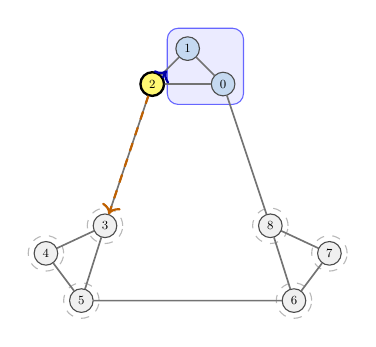
\begin{tikzpicture}[scale=0.5, transform shape,
            vtx/.style={circle, draw=black!70, fill=gray!12, minimum size=6mm, inner sep=0pt, font=\small},
            ed/.style={draw=black!55, semithick},
            sing/.style={draw=gray!55, dashed, circle, minimum size=9mm}]
            \node[vtx, fill=cBlue] (1) at (0,4)       {1};
            \node[vtx, fill=cBlue] (0) at (0.9,3.1)   {0};
            \node[vtx, fill=yellow!55, draw=black, line width=0.3mm] (2) at (-0.9,3.1) {2};
            \node[vtx] (3) at (-2.1,-0.5) {3};
            \node[vtx] (4) at (-3.6,-1.2) {4};
            \node[vtx] (5) at (-2.7,-2.4) {5};
            \node[vtx] (8) at (2.1,-0.5)  {8};
            \node[vtx] (7) at (3.6,-1.2)  {7};
            \node[vtx] (6) at (2.7,-2.4)  {6};
            \draw[ed] (0)--(1) (1)--(2) (2)--(0);
            \draw[ed] (3)--(4) (4)--(5) (5)--(3);
            \draw[ed] (6)--(7) (7)--(8) (8)--(6);
            \draw[ed] (2)--(3) (5)--(6) (8)--(0);
            \begin{scope}[on background layer]
                \foreach \n in {3,4,5,8,7,6} { \node[sing] at (\n) {}; }
                \node[draw=blue!60, fill=blue!8, rounded corners, inner sep=3pt, fit=(0)(1)] (comm01) {};
            \end{scope}
            \draw[->, blue!65!black, thick] (2) to[bend left=12] (comm01);
            \draw[->, orange!75!black, thick, dashed] (2) -- (3);
        \end{tikzpicture}
    \end{columns}
\end{frame}

\begin{frame}{Worked Example (4/6) - Local Moving (continued)}
    \begin{columns}
        \column{0.46\textwidth}
        Node 2 joined, so $\{0,1,2\}$ - the whole top triangle - is now one community.
        \vspace{0.5em}

        The local-moving phase \textbf{keeps going}, visiting the remaining nodes $3$--$8$ the
        same way: each is pulled in by its strong intra-triangle edges, while the single
        bridges are too weak to merge triangles.
        \vspace{0.5em}

        The pass ends once no node can improve $Q$.
        \column{0.54\textwidth}
        \centering
        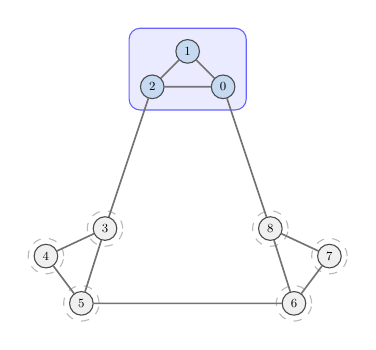
\begin{tikzpicture}[scale=0.5, transform shape,
            vtx/.style={circle, draw=black!70, fill=gray!12, minimum size=6mm, inner sep=0pt, font=\small},
            ed/.style={draw=black!55, semithick},
            sing/.style={draw=gray!55, dashed, circle, minimum size=9mm}]
            \node[vtx, fill=cBlue] (1) at (0,4)       {1};
            \node[vtx, fill=cBlue] (2) at (-0.9,3.1)  {2};
            \node[vtx, fill=cBlue] (0) at (0.9,3.1)   {0};
            \node[vtx] (3) at (-2.1,-0.5) {3};
            \node[vtx] (4) at (-3.6,-1.2) {4};
            \node[vtx] (5) at (-2.7,-2.4) {5};
            \node[vtx] (8) at (2.1,-0.5)  {8};
            \node[vtx] (7) at (3.6,-1.2)  {7};
            \node[vtx] (6) at (2.7,-2.4)  {6};
            \draw[ed] (0)--(1) (1)--(2) (2)--(0);
            \draw[ed] (3)--(4) (4)--(5) (5)--(3);
            \draw[ed] (6)--(7) (7)--(8) (8)--(6);
            \draw[ed] (2)--(3) (5)--(6) (8)--(0);
            \begin{scope}[on background layer]
                \foreach \n in {3,4,5,8,7,6} { \node[sing] at (\n) {}; }
                \node[draw=blue!60, fill=blue!8, rounded corners, inner sep=4pt, fit=(0)(1)(2)] {};
            \end{scope}
        \end{tikzpicture}
    \end{columns}
\end{frame}

\begin{frame}{Worked Example (5/6) - Aggregation}
    \centering
    Local moving ends with \textbf{three communities}, each a triangle ($\Sigma_{in}=3$, total
    degree $8$), giving $Q\approx0.42$. Each community now \textbf{contracts into a super-node}:
    \vspace{0.2em}
    \begin{columns}[c]
        \column{0.5\textwidth}
        \centering
        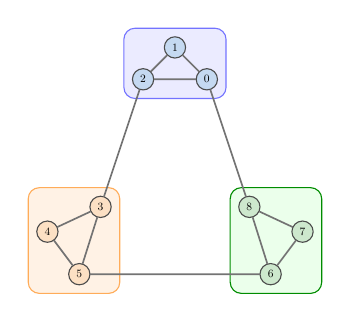
\begin{tikzpicture}[scale=0.45, transform shape,
            vtx/.style={circle, draw=black!70, minimum size=6mm, inner sep=0pt, font=\small},
            ed/.style={draw=black!55, semithick}]
            \node[vtx, fill=cBlue]   (1) at (0,4)       {1};
            \node[vtx, fill=cBlue]   (2) at (-0.9,3.1)  {2};
            \node[vtx, fill=cBlue]   (0) at (0.9,3.1)   {0};
            \node[vtx, fill=cOrange] (3) at (-2.1,-0.5) {3};
            \node[vtx, fill=cOrange] (4) at (-3.6,-1.2) {4};
            \node[vtx, fill=cOrange] (5) at (-2.7,-2.4) {5};
            \node[vtx, fill=cGreen]  (8) at (2.1,-0.5)  {8};
            \node[vtx, fill=cGreen]  (7) at (3.6,-1.2)  {7};
            \node[vtx, fill=cGreen]  (6) at (2.7,-2.4)  {6};
            \draw[ed] (0)--(1) (1)--(2) (2)--(0);
            \draw[ed] (3)--(4) (4)--(5) (5)--(3);
            \draw[ed] (6)--(7) (7)--(8) (8)--(6);
            \draw[ed] (2)--(3) (5)--(6) (8)--(0);
            \begin{scope}[on background layer]
              \node[draw=blue!55, fill=blue!8, rounded corners, inner sep=3pt, fit=(0)(1)(2)] {};
              \node[draw=orange!65, fill=orange!10, rounded corners, inner sep=3pt, fit=(3)(4)(5)] {};
              \node[draw=green!55!black, fill=green!8, rounded corners, inner sep=3pt, fit=(6)(7)(8)] {};
            \end{scope}
        \end{tikzpicture}
        \column{0.06\textwidth}
        \centering\Large $\Rightarrow$
        \column{0.44\textwidth}
        \centering
        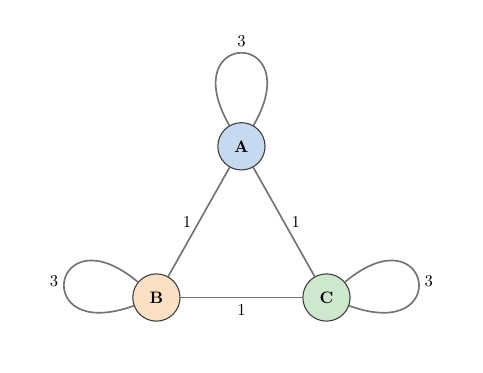
\begin{tikzpicture}[scale=0.6, transform shape,
            sn/.style={circle, draw=black!75, minimum size=10mm, inner sep=0pt, font=\bfseries},
            ed/.style={draw=black!55, semithick}]
            \node[sn, fill=cBlue]   (A) at (0,2.2)   {A};
            \node[sn, fill=cOrange] (B) at (-1.8,-1) {B};
            \node[sn, fill=cGreen]  (C) at (1.8,-1)  {C};
            \draw[ed] (A)--(B) node[midway, left=1pt]  {1};
            \draw[ed] (B)--(C) node[midway, below=1pt] {1};
            \draw[ed] (C)--(A) node[midway, right=1pt] {1};
            \draw[ed] (A) to[out=60, in=120, looseness=12]  node[above]{3} (A);
            \draw[ed] (B) to[out=200, in=140, looseness=12] node[left]{3}  (B);
            \draw[ed] (C) to[out=-20, in=40, looseness=12]  node[right]{3} (C);
        \end{tikzpicture}
    \end{columns}
    \vspace{0.2em}
    {\footnotesize Three internal edges $\to$ a \textbf{self-loop} (weight 3); each bridge $\to$ a unit edge.}
\end{frame}

\begin{frame}{Worked Example (6/6) - Next Level: No Improvement}
    \begin{columns}
        \column{0.5\textwidth}
        \small
        A second local-moving pass starts on the 3-node graph - each super-node is again its
        \textbf{own community} (dashed). \textbf{A} tries to move to \textbf{B} or \textbf{C}:
        \[
            \Delta Q_{A\to B}=\tfrac{1}{12}\!\left[1-\tfrac{8\cdot8}{24}\right]
            = -\tfrac{5}{36}\approx -0.139 < 0
        \]
        (and $\Delta Q_{A\to C}$ is the same). The heavy self-loops outweigh the single
        bridges, so \textbf{no move improves $Q$}.
        \vspace{0.3em}

        \begin{block}{\footnotesize Converged}
        \footnotesize No vertex moves $\Rightarrow$ the algorithm \textbf{stops} with
        \textbf{three communities}, $Q\approx 0.42$.
        \end{block}
        \column{0.5\textwidth}
        \centering
        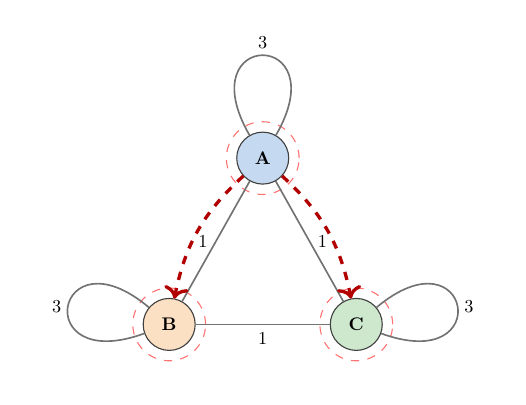
\begin{tikzpicture}[scale=0.66, transform shape,
            sn/.style={circle, draw=black!75, minimum size=10mm, inner sep=0pt, font=\bfseries},
            ed/.style={draw=black!55, semithick},
            sing/.style={draw=red!55, dashed, circle, minimum size=14mm}]
            \node[sn, fill=cBlue]   (A) at (0,2.2)   {A};
            \node[sn, fill=cOrange] (B) at (-1.8,-1) {B};
            \node[sn, fill=cGreen]  (C) at (1.8,-1)  {C};
            \draw[ed] (A)--(B) node[midway, left=1pt]  {1};
            \draw[ed] (B)--(C) node[midway, below=1pt] {1};
            \draw[ed] (C)--(A) node[midway, right=1pt] {1};
            \draw[ed] (A) to[out=60, in=120, looseness=12]  node[above]{3} (A);
            \draw[ed] (B) to[out=200, in=140, looseness=12] node[left]{3}  (B);
            \draw[ed] (C) to[out=-20, in=40, looseness=12]  node[right]{3} (C);
            \begin{scope}[on background layer]
                \node[sing] at (A) {};
                \node[sing] at (B) {};
                \node[sing] at (C) {};
            \end{scope}
            \draw[->, red!70!black, very thick, dashed] (A) to[bend right=18] (B);
            \draw[->, red!70!black, very thick, dashed] (A) to[bend left=18]  (C);
        \end{tikzpicture}
    \end{columns}
\end{frame}

% ============================================================
\section{GPUs \& CUDA}
% ============================================================

\begin{frame}{GPUs: Built for Throughput}
    \begin{columns}
        \column{0.52\textwidth}
        \begin{itemize}
            \item A handful of fast CPU cores vs \textbf{thousands of simple GPU cores} running
            \textbf{thousands of threads} at once.
            \item All that compute is exactly why \textbf{we want to run Louvain on the GPU}.
        \end{itemize}
        \column{0.48\textwidth}
        \centering
        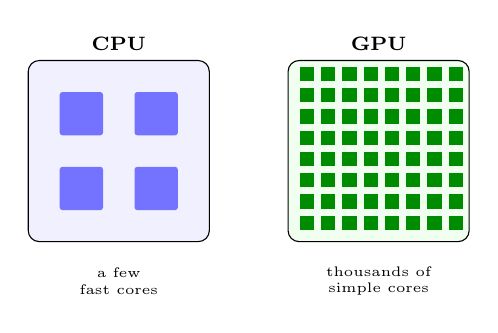
\begin{tikzpicture}[font=\scriptsize]
            % CPU: a few big cores
            \node[draw, rounded corners, fill=blue!6, minimum width=2.3cm, minimum height=2.3cm,
                  label=above:\textbf{CPU}] at (0,0) {};
            \foreach \i in {0,1} \foreach \j in {0,1}
                \fill[blue!55, rounded corners=1pt] (-0.75+\i*0.95, -0.75+\j*0.95) rectangle +(0.55,0.55);
            \node[font=\tiny, align=center] at (0,-1.65) {a few\\fast cores};
            % GPU: thousands of tiny cores
            \node[draw, rounded corners, fill=green!6, minimum width=2.3cm, minimum height=2.3cm,
                  label=above:\textbf{GPU}] at (3.3,0) {};
            \foreach \i in {0,...,7} \foreach \j in {0,...,7}
                \fill[green!55!black] (2.3+\i*0.27, -1.0+\j*0.27) rectangle +(0.18,0.18);
            \node[font=\tiny, align=center] at (3.3,-1.65) {thousands of\\simple cores};
        \end{tikzpicture}
    \end{columns}
\end{frame}

\begin{frame}[fragile]{CUDA Powers It}
    \begin{columns}
        \column{0.44\textwidth}
        \begin{itemize}
            \item \textbf{CUDA} is NVIDIA's programming model for turning that hardware loose.
            \item You write a \textbf{kernel} - a C/C++ function run by \textbf{thousands of
            threads} at once.
            \item Launch it with \texttt{<<<grid, block>>>}; here one block of 32 threads, each
            printing once.
        \end{itemize}
        \column{0.56\textwidth}
        \begin{exampleblock}{The CUDA ``Hello World''}
{\scriptsize
\begin{verbatim}
__global__ void dkernel() {
    printf("Hello World\n");
}

int main() {
    dim3 grid(1, 1, 1);
    dim3 block(32, 1, 1);
    dkernel<<<grid, block>>>();
    cudaDeviceSynchronize();
}
\end{verbatim}
}
        \end{exampleblock}
    \end{columns}
\end{frame}

% ============================================================
\section{Dynamic Community Detection}
% ============================================================

\begin{frame}{Real Networks Keep Changing}
    \begin{columns}
        \column{0.56\textwidth}
        Classic Louvain assumes a \textbf{fixed snapshot}. But real graphs \textbf{never stop
        changing} - vertices and edges arrive and disappear all the time:
        \begin{itemize}
            \item new roads added to a city;
            \item new accounts, new friendships, banned users on social media;
            \item new papers entering a citation database;
            \item updated protein-interaction findings.
        \end{itemize}
        \vspace{0.3em}
        Each update is a \textbf{batch} of edge insertions / deletions, taking
        $G^{t-1} \to G^{t}$.
        \column{0.44\textwidth}
        \centering
        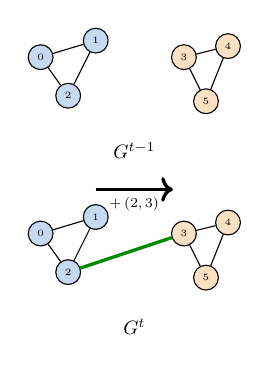
\begin{tikzpicture}[scale=0.7, transform shape,
            v/.style={circle, draw, minimum size=4.5mm, inner sep=0pt, font=\tiny}]
            \foreach \i/\x/\y/\c in {0/0/2/cBlue,1/1/2.3/cBlue,2/0.5/1.3/cBlue,
                                     3/2.6/2/cOrange,4/3.4/2.2/cOrange,5/3/1.2/cOrange}{
                \node[v, fill=\c] (\i) at (\x,\y) {\i};}
            \draw (0)--(1) (1)--(2) (2)--(0)  (3)--(4) (4)--(5) (5)--(3);
            \node at (1.7,0.3) {$G^{t-1}$};
            \draw[->, very thick] (1.0,-0.4) -- (2.4,-0.4)
                node[midway, below, font=\scriptsize] {$+\,(2,3)$};
            \begin{scope}[yshift=-3.2cm]
            \foreach \i/\x/\y/\c in {0/0/2/cBlue,1/1/2.3/cBlue,2/0.5/1.3/cBlue,
                                     3/2.6/2/cOrange,4/3.4/2.2/cOrange,5/3/1.2/cOrange}{
                \node[v, fill=\c] (b\i) at (\x,\y) {\i};}
            \draw (b0)--(b1) (b1)--(b2) (b2)--(b0)  (b3)--(b4) (b4)--(b5) (b5)--(b3);
            \draw[green!55!black, very thick] (b2)--(b3);
            \node at (1.7,0.3) {$G^{t}$};
            \end{scope}
        \end{tikzpicture}
    \end{columns}
\end{frame}

\begin{frame}{\dots and the Graphs are Huge}
    \textbf{Researchers already run \emph{Louvain} on exactly these massive, evolving graphs:}
    \vspace{0.6em}
    \begin{itemize}
        \item \textbf{Twitter / X during the 2022 Ukraine war} - a communication graph of
        \textbf{3.2\,M users / 27.4\,M edges}; pro/anti factions form and shift over the first
        four weeks. Communities are detected with \textbf{Louvain} (and compared against
        Leiden).\\[-0.1em]
        {\scriptsize\itshape \'Sliwa, Ku\v{s}en, Strembeck - ``Comparing Twitter Communities
        by Louvain \& Leiden during the 2022 War in Ukraine'', WWW '24 Companion.}
        \item \textbf{Opinion communities on Reddit} reorganise over months and years -
        again tracked using \textbf{Louvain} community detection.\\[-0.1em]
        {\scriptsize\itshape Reddit opinion-dynamics study, \emph{Information Sciences}, 2026.}
    \end{itemize}
    \vspace{0.6em}
    \begin{center}
    Millions of edges \textbf{+} a new batch arriving constantly
    $\;\Rightarrow\;$ re-running static Louvain every time is \textbf{infeasible}.
    \end{center}
\end{frame}

\begin{frame}{The Problem - and the Gap We Fill}
    \begin{columns}
        \column{0.6\textwidth}
        \begin{itemize}
            \item The classic \textbf{Louvain} method is built for a \textbf{single static
            snapshot}.
            \item On a changing graph the usual practice is to \textbf{re-run it from scratch}
            after every update - prohibitive at scale and frequency.
            \item \textbf{Dynamic} variants instead \textbf{update incrementally} from the
            previous partition.
            \item On \textbf{GPUs}, fast static Louvain exists (cuGraph, cuVite, Nido) - but
            a \textbf{dynamic GPU} implementation is almost unexplored.
        \end{itemize}
        \column{0.4\textwidth}
        \begin{alertblock}{This project}
        A from-scratch CUDA \textbf{GPU dynamic Louvain}: a corrected static algorithm
        \emph{plus} three incremental variants (ND, DS, DF), benchmarked against
        cuGraph, NetworKit and NetworkX.
        \end{alertblock}
    \end{columns}
\end{frame}

\begin{frame}{The Research Landscape - Where We Sit}
    \centering
    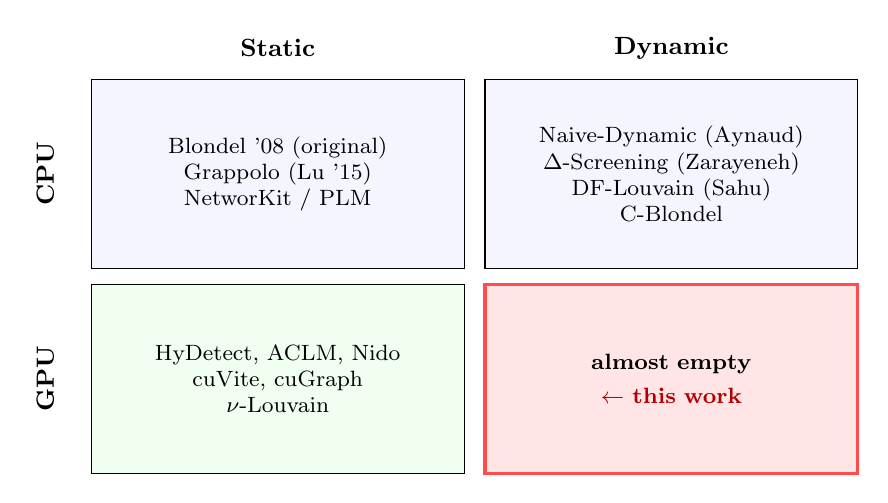
\begin{tikzpicture}[font=\footnotesize,
        cell/.style={draw, minimum width=4.7cm, minimum height=2.4cm, align=center, text width=4.5cm},
        hd/.style={font=\small\bfseries}]
        \node[hd] at (2.55,2.0) {Static};
        \node[hd] at (7.55,2.0) {Dynamic};
        \node[hd, rotate=90] at (-0.4,0.4) {CPU};
        \node[hd, rotate=90] at (-0.4,-2.2) {GPU};
        % CPU-static
        \node[cell, fill=blue!4] at (2.55,0.4)
            {Blondel '08 (original)\\ Grappolo (Lu '15)\\ NetworKit / PLM};
        % CPU-dynamic
        \node[cell, fill=blue!4] at (7.55,0.4)
            {Naive-Dynamic (Aynaud)\\ $\Delta$-Screening (Zarayeneh)\\ DF-Louvain (Sahu)\\ C-Blondel};
        % GPU-static
        \node[cell, fill=green!6] at (2.55,-2.2)
            {HyDetect, ACLM, Nido\\ cuVite, cuGraph\\ $\nu$-Louvain};
        % GPU-dynamic (the gap)
        \node[cell, fill=red!10, very thick, draw=red!70] at (7.55,-2.2)
            {\textbf{almost empty}\\[0.3em]
             \textcolor{red!70!black}{\textbf{$\leftarrow$ this work}}};
    \end{tikzpicture}
    \\[0.5em]
    {\small Interesting find from the survey: \textbf{Leiden} often beats Louvain in quality
    (cf.\ the Ukraine study) - a natural future direction.}
\end{frame}

\begin{frame}{From Static to Dynamic}
    Static Louvain is run \textbf{once} on the initial graph. After that, updates arrive as
    \textbf{batches} - each batch is a set of edge \textbf{deletions and additions}.
    The two phases are unchanged; dynamic Louvain differs in just \textbf{two} ways:
    \begin{itemize}
        \item \textbf{Warm start.} Start each node from its community in the \emph{previous}
        partition (not singletons) - already near-optimal, so few moves are needed.
        \item \textbf{Affected vertices.} Only process the nodes whose community might change;
        the rest stay put.
    \end{itemize}
    \begin{alertblock}{The central design choice = the \emph{affected set}}
    Too small $\Rightarrow$ miss moves, quality drops. \quad
    Too large $\Rightarrow$ a lot more compute than needed.
    \end{alertblock}
\end{frame}

\begin{frame}{Three Ways to Mark the Affected Set}
    \centering
    \vspace{0.8em}
    \small
    \begin{tabular}{@{}p{1.6cm}p{4.7cm}p{5.6cm}@{}}
        \toprule
        \textbf{Variant} & \textbf{Affected set} & \textbf{How it is found} \\
        \midrule
        \textbf{ND} & every vertex & warm start only; no locality \\[0.5em]
        \textbf{DS} & fixed superset, up front & screen by $\Delta Q$: mark endpoint, its
            neighbours \& the whole target/source community \\[0.5em]
        \textbf{DF} & minimal seed that grows & mark changed endpoints; when a vertex moves,
            mark its neighbours \\
        \bottomrule
    \end{tabular}
\end{frame}

% ============================================================
\section{Implementation, Challenges \& Results}
% ============================================================

\begin{frame}{Data Structures}
    \begin{columns}[T]
        \column{0.52\textwidth}
        \textbf{Graph - Compressed Sparse Row (CSR)}
        \begin{itemize}\small
            \item Real graphs are \textbf{sparse} ($|E|\ll|V|^2$) - an adjacency matrix is
            hopeless.
            \item An \texttt{offset} array + a flat \texttt{neighbour} array; vertex $v$'s
            neighbours are the range \texttt{[off[v], off[v{+}1])}.
            \item Memory $O(|V|+|E|)$; coalesced, $O(1)$ access to a neighbour list.
        \end{itemize}
        \vspace{0.2em}
        \centering
        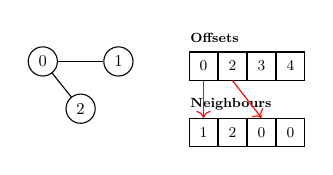
\begin{tikzpicture}[scale=0.6, transform shape,
            arr/.style={draw, minimum size=0.6cm, inner sep=1pt, font=\small}]
            \node[circle, draw] (A) at (0,1) {0};
            \node[circle, draw] (B) at (1.6,1) {1};
            \node[circle, draw] (C) at (0.8,0) {2};
            \draw (A)--(B); \draw (A)--(C);
            \node[anchor=west, font=\footnotesize] at (3.0,1.5) {\textbf{Offsets}};
            \node[arr] (o0) at (3.4,0.9) {0};
            \node[arr, right=0pt of o0] (o1) {2};
            \node[arr, right=0pt of o1] (o2) {3};
            \node[arr, right=0pt of o2] (o3) {4};
            \node[anchor=west, font=\footnotesize] at (3.0,0.1) {\textbf{Neighbours}};
            \node[arr] (e0) at (3.4,-0.5) {1};
            \node[arr, right=0pt of e0] (e1) {2};
            \node[arr, right=0pt of e1] (e2) {0};
            \node[arr, right=0pt of e2] (e3) {0};
            \draw[->, red] (o0.south) -- (e0.north);
            \draw[->, red] (o1.south) -- (e2.north);
        \end{tikzpicture}
        \column{0.48\textwidth}
        \textbf{Per-vertex hashtable}
        \begin{itemize}\small
            \item Choosing a vertex's best community needs its \textbf{weight to each
            neighbouring community}.
            \item Each vertex owns a \textbf{private open-addressing hashtable} (keyed by
            community), sized to its degree - so accumulation needs \textbf{no locks}.
            \item Held in one global \texttt{htKey}/\texttt{htVal} pair, split per vertex by a
            prefix-sum offset array.
        \end{itemize}
        \vspace{0.3em}
        Plus length-$|V|$ state arrays: community \texttt{C}, degree \texttt{K}, community
        totals $\Sigma$, and the \texttt{active}/\texttt{range} masks.
    \end{columns}
\end{frame}

\begin{frame}{The Local-Moving Kernel: Verified Commit Under Lock}
    One GPU thread per vertex $v$, in \textbf{four steps}:
    \begin{enumerate}\small
        \item \textbf{Accumulate} - add $v$'s edge weight to each neighbouring community in
        its hashtable slice.
        \item \textbf{Optimistic pick} - choose \texttt{best\_c} with the largest gain,
        reading $\Sigma$ \emph{optimistically} (may be stale).
        \item \textbf{Lock} the \textbf{community pair} $(d,\texttt{best\_c})$, lower id first
        (deadlock-free).
        \item \textbf{Verify \& commit} - with both communities frozen, recompute the
        \emph{exact} $\Delta Q$ and move \textbf{only if it is still positive}.
    \end{enumerate}
    \vspace{0.3em}
    \begin{exampleblock}{Why it is correct}
    Holding both community locks during verification means no other thread can change either
    community's membership $\Rightarrow$ \textbf{every committed move provably increases
    modularity} (no stale-$\Sigma$ moves, no 2-cycle swaps).
    \end{exampleblock}
\end{frame}

\begin{frame}{One Driver}
    \begin{columns}
        \column{0.56\textwidth}
        \begin{itemize}
            \item A \textbf{single shared multi-level driver} runs the \textbf{static pass} and
            \textbf{all three dynamic variants} (ND, DS, DF).
            \item They differ only in two inputs: the \textbf{warm-start community labels} and
            the initial \texttt{active}/\texttt{range} masks.
            \item Each level alternates the \textbf{local-moving kernel} with \textbf{Thrust
            aggregation}, then repeats on the coarser graph until the partition stops improving.
        \end{itemize}
        \column{0.44\textwidth}
        \centering
        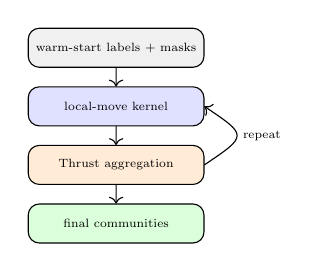
\begin{tikzpicture}[scale=0.62, transform shape, font=\scriptsize,
            b/.style={draw, rounded corners, minimum width=3.6cm, minimum height=0.8cm}]
            \node[b, fill=gray!12] (in) at (0,3.0) {warm-start labels + masks};
            \node[b, fill=blue!12] (lm) at (0,1.8) {local-move kernel};
            \node[b, fill=orange!16] (ag) at (0,0.6) {Thrust aggregation};
            \node[b, fill=green!14] (out) at (0,-0.6) {final communities};
            \draw[->] (in)--(lm); \draw[->] (lm)--(ag); \draw[->] (ag)--(out);
            \draw[->] (ag.east) .. controls (2.7,1.2) .. (lm.east)
                node[midway,right]{repeat};
        \end{tikzpicture}
    \end{columns}
\end{frame}

\begin{frame}{Improvements since UGRC}
    \small
    The UGRC predecessor \emph{``collapsed into a single community \dots likely a
    synchronization error''} - it did so \textbf{sometimes, on large graphs}. We traced and
    fixed exactly this:
    \begin{itemize}
        \item \textbf{Self-loop $\Delta Q$ bug.} After aggregation every super-node has a large
        self-loop; the old gain wrongly counted it $\Rightarrow$ inflated gains $\Rightarrow$
        \textbf{communities collapsed} from pass 2 onward. \emph{Fix:} skip the self-loop.
        \item \textbf{Float-noise thrashing.} Near-zero equal-and-opposite gains kept passes
        oscillating. \emph{Fix:} a strict positivity threshold \texttt{MOVE\_EPS} ($10^{-12}$).
    \end{itemize}
    \centering\textbf{Result:} modularity is now non-decreasing. No collapse.
\end{frame}

\begin{frame}{Challenges}
    \begin{itemize}
        \item \textbf{Edge-parallel $\to$ vertex-parallel.} UGRC split the arc array and needed
        \textbf{four spin-locks} per move. This change required some rework.
        \vspace{0.5em}
        \item \textbf{A per-vertex hash table.} I did not consider this initially but saw it in a paper. This is to store weight of edges to each neighbour of a vertex - required for gain calculations.
        \vspace{0.5em}
        \item \textbf{Cooperative kernels $\to$ per-iteration relaunch.} \texttt{grid.sync()}
        needs all blocks co-resident ($\approx$48 on my RTX3050) - can't fit millions of
        vertices. Now the \textbf{host relaunches} the kernel each iteration; the launch
        boundary \emph{is} the global barrier $\Rightarrow$ scales to any size.
    \end{itemize}
\end{frame}

\begin{frame}{An Optimisation}
    \begin{itemize}
        \item \textbf{Coalesced memory access.} The graph is stored as a
        \textbf{structure-of-arrays}, so the $32$ lanes of a warp read \textbf{adjacent words}
        in a single memory transaction - rather than strided reads from an
        array-of-structures.
    \end{itemize}
\end{frame}

\begin{frame}{An Interesting Find}
    \begin{itemize}
        \item The \emph{same} source \textbf{hangs on sm\_60} (pre-Volta) but runs in
        \textbf{milliseconds on sm\_86}. The community-pair locks rely on Volta+
        \textbf{Independent Thread Scheduling}, where the lanes of a warp make independent
        progress.
    \end{itemize}
\end{frame}

\begin{frame}{Experimental Setup}
    \begin{columns}
        \column{0.5\textwidth}
        \textbf{Hardware (Google Colab)}
        \begin{itemize}\small
            \item \textbf{NVIDIA T4} (15\,GB) - most graphs
            \item \textbf{NVIDIA A100} (40\,GB) - the two largest
        \end{itemize}
        \textbf{Baselines}
        \begin{itemize}\small
            \item \textbf{NetworkX} - single-thread CPU
            \item \textbf{NetworKit} - parallel CPU (PLM)
            \item \textbf{cuGraph} - GPU (RAPIDS)
        \end{itemize}
        \column{0.5\textwidth}
        \textbf{Graphs} (common format; undirected, unit weight)
        \begin{itemize}\small
            \item 2 classic (karate, dolphins) - correctness
            \item \textbf{12 SNAP static}: 4\,K--3\,M vertices,
            88\,K--\textbf{117\,M} edges
            \item \textbf{4 SNAP temporal}: 80\% initial + $5\times4\%$ insertion batches
            \item synthetic churn on com-DBLP (quality)
        \end{itemize}
        \textbf{Metrics:} modularity, \# communities, wall-clock time.
    \end{columns}
\end{frame}

\begin{frame}{Static - Performance}
    \begin{columns}
        \column{0.54\textwidth}
        \centering
        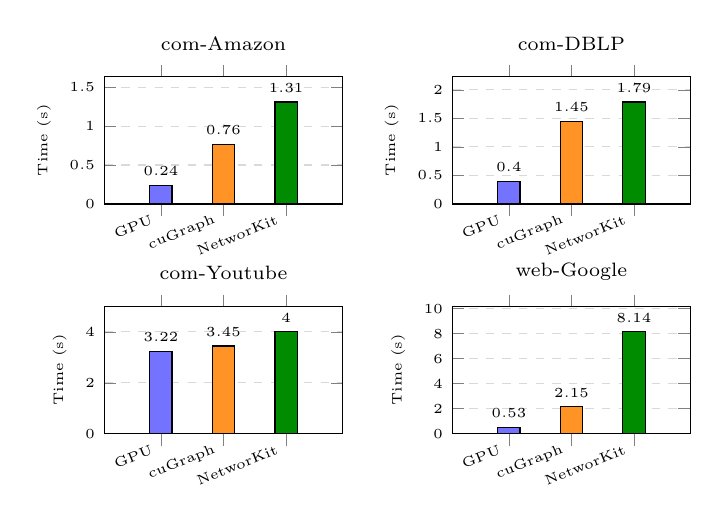
\begin{tikzpicture}
        \begin{groupplot}[
            group style={group size=2 by 2, horizontal sep=1.4cm, vertical sep=1.3cm},
            width=4.6cm, height=3.2cm, ybar, ymin=0,
            enlarge y limits={upper, value=0.25}, enlarge x limits=0.45,
            symbolic x coords={GPU,cuGraph,NetworKit},
            xtick={GPU,cuGraph,NetworKit},  % explicit: xtick=data only caught the first bar
            x tick label style={rotate=22, anchor=east, font=\tiny},
            y tick label style={font=\tiny}, ylabel={Time (s)},
            ylabel style={font=\tiny}, title style={font=\scriptsize},
            ymajorgrids=true, grid style={dashed, gray!30},
            nodes near coords, nodes near coords style={font=\tiny},
            every axis plot/.append style={bar width=8pt, bar shift=0pt}]
        \nextgroupplot[title={com-Amazon}]
        \addplot[fill=blue!55] coordinates {(GPU,0.242)};
        \addplot[fill=orange!85] coordinates {(cuGraph,0.763)};
        \addplot[fill=green!55!black] coordinates {(NetworKit,1.309)};
        \nextgroupplot[title={com-DBLP}]
        \addplot[fill=blue!55] coordinates {(GPU,0.397)};
        \addplot[fill=orange!85] coordinates {(cuGraph,1.452)};
        \addplot[fill=green!55!black] coordinates {(NetworKit,1.787)};
        \nextgroupplot[title={com-Youtube}]
        \addplot[fill=blue!55] coordinates {(GPU,3.223)};
        \addplot[fill=orange!85] coordinates {(cuGraph,3.447)};
        \addplot[fill=green!55!black] coordinates {(NetworKit,4.003)};
        \nextgroupplot[title={web-Google}]
        \addplot[fill=blue!55] coordinates {(GPU,0.532)};
        \addplot[fill=orange!85] coordinates {(cuGraph,2.154)};
        \addplot[fill=green!55!black] coordinates {(NetworKit,8.143)};
        \end{groupplot}
        \end{tikzpicture}
        \column{0.46\textwidth}
        \begin{itemize}\small
            \item All four implementations reach \textbf{essentially the same modularity}.
            \item These are four of the largest SNAP graphs.
        \end{itemize}
        \begin{block}{Headline (six largest SNAP)}
        \small geo-mean \textbf{1.74$\times$} vs cuGraph, \textbf{2.18$\times$} vs NetworKit.\\[0.2em]
        \textbf{web-Google} (4.3\,M edges): 0.53\,s =
        \textbf{4$\times$ / 15$\times$ / 450$\times$} vs cuGraph / NetworKit / NetworkX.
        \end{block}
    \end{columns}
\end{frame}

\begin{frame}{Static - Why hubs are reducing performance}
    \footnotesize
    \begin{center}
    \begin{tabular}{lrrrrcc}
        \toprule
        \textbf{Graph} & $|V|$ & $|E|$ & \textbf{Avg} & \textbf{Max} &
        \textbf{vs cuGraph} & \textbf{vs NetworKit} \\
        \midrule
        com-DBLP        & 317{,}080  & 1{,}049{,}866   & 6.6  & 343    & \win{3.66$\times$} & \win{4.50$\times$} \\
        com-Amazon      & 334{,}863  & 925{,}872       & 5.5  & 549    & \win{3.15$\times$} & \win{5.41$\times$} \\
        web-Google      & 875{,}713  & 4{,}322{,}051   & 9.9  & 6{,}332 & \win{4.05$\times$} & \win{15.31$\times$} \\
        \midrule
        com-Youtube     & 1{,}134{,}890 & 2{,}987{,}624 & 5.3 & 28{,}754 & 1.07$\times$ & 1.24$\times$ \\
        com-LiveJournal & 3{,}997{,}962 & 34{,}681{,}189 & 17.4 & 14{,}815 & 1.03$\times$ & \loss{0.81$\times$} \\
        com-Orkut       & 3{,}072{,}441 & 117{,}185{,}083 & 76.3 & 33{,}313 & \loss{0.54$\times$} & \loss{0.29$\times$} \\
        \bottomrule
    \end{tabular}
    \end{center}
    \begin{columns}
        \column{0.62\textwidth}
        \begin{itemize}\small
            \item The split tracks \textbf{maximum degree}: bounded-degree graphs win big;
            \textbf{hub-dominated} social graphs collapse the advantage.
            \item \textbf{Why:} a \emph{vertex-parallel} warp stalls when 31 lanes finish and
            one holds a degree-33{,}000 hub - classic load imbalance.
        \end{itemize}
        \column{0.38\textwidth}
    \end{columns}
\end{frame}

\begin{frame}{Dynamic - Incremental Updates are Far Faster}
`    \footnotesize
    \begin{center}
    \begin{tabular}{lrrrrrr}
        \toprule
        \textbf{Avg.\ per-batch time (ms)} & \textbf{ND} & \win{\textbf{DF}} & \textbf{DS}
            & \textbf{cuGraph} & \textbf{NetworKit} & \textbf{NetworkX} \\
        \midrule
        CollegeMsg       & 1.2  & \win{0.4}  & 1.2   & 64.8  & 3.3   & 312.5 \\
        sx-mathoverflow  & 50.0 & \win{23.6} & 49.6  & 264.5 & 73.3  & 6{,}176.0 \\
        sx-askubuntu     & 68.6 & \win{49.8} & 109.2 & 439.3 & 288.6 & 32{,}476.4 \\
        sx-superuser     & 95.6 & \win{66.4} & 96.2  & 682.0 & 434.4 & 45{,}998.0 \\
        \bottomrule
    \end{tabular}
    \end{center}
    \vspace{0.2em}
    \begin{columns}
        \column{0.54\textwidth}
        \begin{itemize}\small
            \item Baselines must \textbf{re-cluster the whole graph} every batch; our variants
            reprocess only the \textbf{affected vertices} from the warm start.
            \item \textbf{DF} touches the smallest set $\Rightarrow$ fastest.
        \end{itemize}
        \column{0.46\textwidth}
        \begin{block}{Headline (DF, 4\% batches, geo-mean)}
        \small \textbf{20.14$\times$} vs cuGraph, \textbf{5.58$\times$} vs NetworKit,
        \textbf{hundreds$\times$} vs NetworkX.
        \end{block}
    \end{columns}
\end{frame}

\begin{frame}{Dynamic - Quality is Preserved}
    \begin{columns}
        \column{0.6\textwidth}
        \centering
        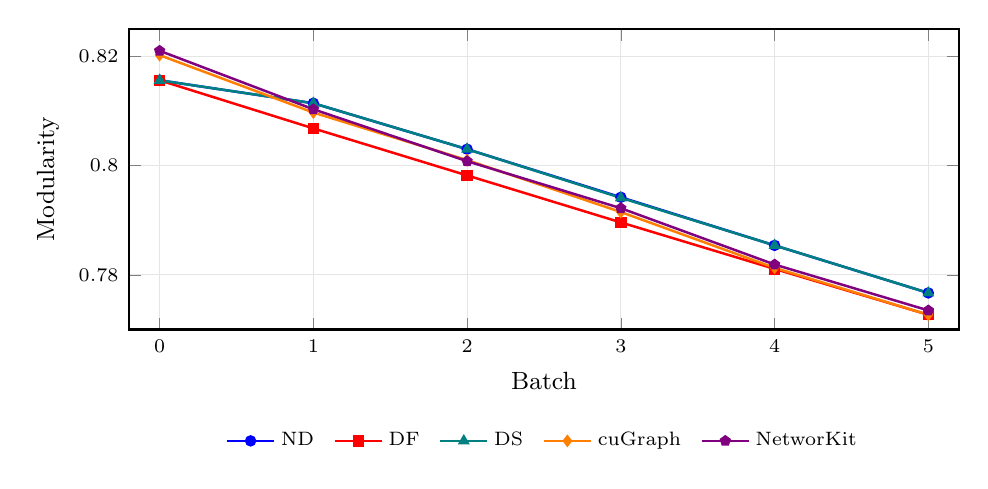
\begin{tikzpicture}
        \begin{axis}[
            width=\textwidth, height=5.4cm,
            xlabel={Batch}, ylabel={Modularity},
            xmin=-0.2, xmax=5.2, xtick={0,1,2,3,4,5},
            ymin=0.770, ymax=0.825,
            grid=both, grid style={gray!20},
            tick label style={font=\scriptsize}, label style={font=\small},
            mark size=1.6pt, line width=0.9pt,
            legend style={at={(0.5,-0.30)}, anchor=north, legend columns=5, draw=none,
                font=\scriptsize, /tikz/every even column/.append style={column sep=5pt}}]
        \addplot[blue, mark=*] coordinates {(0,0.8156)(1,0.8114)(2,0.8030)(3,0.7942)(4,0.7854)(5,0.7767)};
        \addplot[red, mark=square*] coordinates {(0,0.8156)(1,0.8068)(2,0.7982)(3,0.7896)(4,0.7811)(5,0.7727)};
        \addplot[teal, mark=triangle*] coordinates {(0,0.8156)(1,0.8114)(2,0.8030)(3,0.7941)(4,0.7854)(5,0.7767)};
        \addplot[orange, mark=diamond*] coordinates {(0,0.8202)(1,0.8097)(2,0.8010)(3,0.7915)(4,0.7813)(5,0.7727)};
        \addplot[violet, mark=pentagon*] coordinates {(0,0.8210)(1,0.8103)(2,0.8008)(3,0.7922)(4,0.7819)(5,0.7735)};
        \legend{ND, DF, DS, cuGraph, NetworKit}
        \end{axis}
        \end{tikzpicture}
        \column{0.4\textwidth}
        \small
        com-DBLP, synthetic churn (\textbf{60\% insert / 40\% delete}), five cumulative batches.
        \begin{itemize}
            \item All five curves stay \textbf{within $0.01$} at every batch.
            \item Holds even for \textbf{20\%-of-$|E|$} batches.
            \item Incremental variants \textbf{track full re-clustering} - the degradation is
            the \emph{perturbed graph's}, not the method's.
        \end{itemize}
    \end{columns}
\end{frame}

% ============================================================
\section{Conclusion}
% ============================================================

\begin{frame}{Conclusion}
    \begin{itemize}
        \item Built, from scratch in CUDA, a \textbf{GPU dynamic Louvain}: a corrected static
        algorithm + three incremental variants (ND, DS, DF) on \textbf{one shared driver}.
        \item Resolved the UGRC correctness failures - moves are now \textbf{modularity
        non-decreasing}.
        \item \textbf{Static:} reference-quality partitions, with a \textbf{speed-up over
        cuGraph and NetworKit} on large graphs; honest limit on hub-dominated graphs.
        \item \textbf{Dynamic:} \textbf{20$\times$ vs cuGraph}, several$\times$ vs NetworKit,
        hundreds$\times$ vs NetworkX - at \textbf{little to no quality cost}.
        \item To our knowledge, the \textbf{only public GPU dynamic Louvain} apart from
        StarPlat.
    \end{itemize}
\end{frame}

\begin{frame}{Future Work}
    \begin{columns}
        \column{0.5\textwidth}
        \textbf{Algorithmic}
        \begin{itemize}\small
            \item Modify the algorithm to be \textbf{more GPU-specific} (not just a CPU port).
            \item Explicit \textbf{vertex} add/delete.
            \item A dynamic GPU \textbf{Leiden}.
        \end{itemize}
        \column{0.5\textwidth}
        \textbf{Evaluation}
        \begin{itemize}\small
            \item \textbf{NMI / ARI} vs ground truth; modularity density. (I do not know what each is in detail)
            \item Direct \textbf{DF-Louvain} (OpenMP) baseline.
            \item Just keep profiling.
            \item Benchmark: Billions of edges \textbf{uk-2007}; weighted \& real-deletion temporal graphs.
        \end{itemize}
        \vspace{0.3em}
        \textbf{Publication}
        \begin{itemize}\small
            \item Parallel-computing venues: IJPP, JPDC, IEEE TPDS, ICPP.
        \end{itemize}
    \end{columns}
\end{frame}

\begin{frame}
    \centering
    \vfill
    {\Huge \textbf{Q/A?}}\\[1.5em]
    {\small Code: \texttt{github.com/KlowdfurrRad/dynamic\_louvain\_cuda\_\_BTP}}
    \vfill
    {\tiny LLMs were used in slide generation.}
\end{frame}

\end{document}
